\chapter{Experimental Studies}
\label{chap:implementation}

\section{Testbed Overview}
\label{sec:testbed-overview}

Both proofs of concept were executed on the same single-node testbed. Keeping the physical node and GPU software stack fixed reduces environmental variation between the two studies and allows the experiments to reuse the same DRA inventory, monitoring path, and MIG management procedure. Table~\ref{tab:testbed-overview} reports the main components and their role.

\begin{table}[htbp]
    \centering
    \small
    \caption{Experimental testbed configuration.}
    \label{tab:testbed-overview}
    \begin{tabularx}{\textwidth}{@{}p{0.20\textwidth}p{0.37\textwidth}X@{}}
        \toprule
        \textbf{Component} & \textbf{Configuration} & \textbf{Role in the testbed} \\
        \midrule
        Cloud host & Google Cloud virtual machine with an NVIDIA A100 attached through PCIe passthrough & Provides exclusive access to the physical accelerator while retaining a reproducible cloud-hosted environment. \\
        Accelerator & NVIDIA A100-SXM4-40GB, Ampere architecture, 40~GB HBM2, 108 physical SMs & Executes the inference and batch workloads and supports the MIG layouts evaluated in the proofs of concept. \\
        Node software & Ubuntu 24.04.4 LTS and containerd 2.1.5-k3s1 & Supplies the Linux host and OCI container runtime recorded for the experimental node. \\
        Kubernetes & Single-node K3s v1.35.2+k3s1 & Provides the stable DRA API and a controlled scheduler environment. \\
        GPU management & NVIDIA GPU Operator v26.3.0, MIG strategy \texttt{mixed}, MIG Manager enabled & Installs and reconciles the container GPU stack and applies declared MIG geometries. \\
        Device allocation & NVIDIA DRA Driver for GPUs v25.12.0 & Publishes GPU and MIG devices as structured resources and prepares the device selected for each claim. \\
        Observability & \texttt{kube-prometheus-stack}, DCGM Exporter, ServiceMonitor, and a dedicated Grafana dashboard & Scrapes GPU telemetry every five seconds and visualizes utilization, memory, power, temperature, and related health metrics. \\
        \bottomrule
    \end{tabularx}
\end{table}

The physical A100 contains 108 SMs, but MIG organizes its allocatable compute capacity into seven compute slices. On this model each slice contains 14 SMs, so the full-size \texttt{7g.40gb} MIG profile exposes 98 SMs rather than all 108 physical SMs. The experiments use only \texttt{1g.5gb}, \texttt{3g.20gb}, and \texttt{7g.40gb}. This distinction between physical and MIG-addressable SMs is important when interpreting a ``full GPU'' baseline~\cite{nvidia2026gpuperformance,nvidia2026migconcepts}.

The Operator configuration deliberately disables the conventional NVIDIA device plugin so that GPU allocation follows the DRA path. It keeps the NVIDIA Container Toolkit, GPU Feature Discovery, MIG Manager, and DCGM Exporter enabled. MIG Manager is allowed to reboot the node when a mode transition requires it, while the \texttt{mixed} strategy permits heterogeneous profile names to be exposed. Finally, the standalone NVIDIA DRA driver is scheduled on the GPU node. This arrangement matches the separation introduced in Section~\ref{chap:architecture-overview}: the Operator manages node capabilities, whereas the DRA driver implements claim-based allocation.

For observability, DCGM Exporter samples GPU metrics at a five-second interval and exposes them through a Prometheus Operator ServiceMonitor. The \texttt{kube-prometheus-stack} installation stores the resulting time series, and Grafana loads a dedicated dashboard for both full-GPU and MIG views. These measurements complement the application-level timings emitted by the benchmarks. Because the cluster contains one worker/control-plane node and one physical GPU, the experiments evaluate allocation and consolidation on that node, but they do not test cross-node scheduling, high availability, or multi-GPU communication.

\section{PoC 1: Parallel Ollama Instances}
\label{sec:multi-ollama}

The first proof of concept deploys TinyLlama behind one Kubernetes Service using a variable number of independent Ollama inference-server replicas. Its purpose is to determine whether parallel isolated servers can transform capacity left unused by one lightweight workload into useful aggregate throughput. The experiment is intentionally incremental: it first measures one server on the largest available device, then distinguishes the effects of sharing, restricting, and spatially partitioning that resource.

\subsection{Targeted Challenges}
\label{subsec:multi-ollama-problem}

The proof of concept targets two related limitations of a single inference-server deployment:

\begin{description}
    \item[GPU underutilization.] A small or lightweight model may fit comfortably in accelerator memory while failing to keep all SMs active, even when the service is subjected to sustained demand. Assigning an entire high-end GPU to that server then reserves compute and memory capacity that cannot be used by another tenant. TinyLlama, a 1.1-billion-parameter language model, provides a compact LLM workload with which to observe this mismatch~\cite{zhang2024tinyllama}.
    \item[Head-of-line queueing.] An inference server has finite request concurrency. During a spike, requests that exceed the work the server can process concurrently remain queued behind earlier requests. In particular, Ollama can manage only one request per time. Without a mechanism such as effective dynamic batching or additional serving replicas, trailing requests wait for capacity to become available, increasing latency even when the physical GPU still contains exploitable parallel resources. Here, \emph{head-of-line blocking} refers to this application-level queueing effect rather than to a transport-protocol property.
\end{description}

The two problems suggest a common direction: deploy more than one serving process so that requests can be handled by independent workers, while preventing those workers from interfering without control. Merely creating additional processes on the same device tests concurrency but does not provide resource or fault isolation. MIG makes it possible to compare that temporal sharing arrangement with spatially isolated replicas.

\subsection{System Design}
\label{subsec:multi-ollama-architecture}

The system consists of a configurable MIG hardware view, a DRA allocation path, one or more Ollama Pods, a single Kubernetes Service, and an external load generator. Table~\ref{tab:ollama-gpu-views} represents the three device sizes used to construct the four experimental cases. The term \emph{full GPU} is used for readability to denote the full-size \texttt{7g.40gb} MIG device, actually the baseline still uses MIG mode so that every case follows the same DRA resource model.

\begin{figure}[htbp]
    \centering
    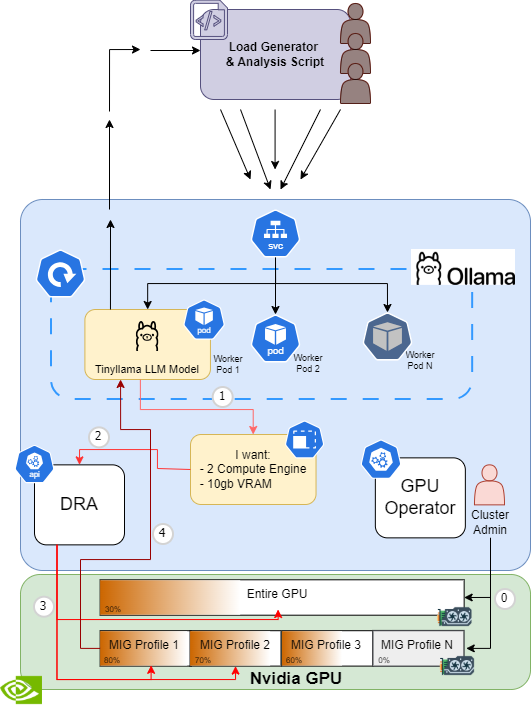
\includegraphics[width=0.8\textwidth]{images/Ollama_testbed.drawio.png}
    \caption{Ollama Experiment System Design}
    \label{fig:esempio}
\end{figure}

\begin{table}[htbp]
    \centering
    \small
    \caption{MIG device views used by the Ollama proof of concept.}
    \label{tab:ollama-gpu-views}
    \begin{tabularx}{\textwidth}{@{}p{0.20\textwidth}p{0.20\textwidth}p{0.16\textwidth}p{0.15\textwidth}X@{}}
        \toprule
        \textbf{Experimental view} & \textbf{MIG device(s) used} & \textbf{SMs per device} & \textbf{Memory per device} & \textbf{Purpose} \\
        \midrule
        Full-size & $1 \times$ \texttt{7g.40gb} & 98 & 40~GB & Whole-resource baseline and shared-device comparison. \\
        Medium & $1 \times$ \texttt{3g.20gb} & 42 & 20~GB & Measures the effect of restricting one server to a fraction of the accelerator. \\
        Small partitions & $7 \times$ \texttt{1g.5gb} & 14 & 5~GB & Provides one isolated device for each of seven parallel servers. \\
        \bottomrule
    \end{tabularx}
\end{table}

The MIG configuration is selected at node level and applied by MIG Manager before a test case begins. At the allocation layer, the proof of concept intentionally uses a generic request. The ResourceClaimTemplate named \texttt{whatever-mig} requests exactly one device from the \texttt{mig.nvidia.com} DeviceClass and applies only the following CEL condition:

\begin{quote}
\texttt{device.attributes["gpu.nvidia.com"].type == "mig"}
\end{quote}

The claim does not select a profile, memory size, or number of SMs. Consequently, the node's pre-applied MIG geometry determines which kind of device can satisfy it. This keeps application manifests independent of a profile name, but it is safe only when the experiment controls the available inventory. A production cluster exposing several acceptable MIG profiles would normally add selectors or use more specific DeviceClasses to avoid an unintended allocation.

The application is defined by the \texttt{ollama-mig} Deployment and each replica runs the \texttt{ollama/ollama:0.12.11-rc1} image. An init container starts a temporary Ollama server and pulls TinyLlama into an \texttt{emptyDir} volume, then the main container subsequently reuses that per-Pod model directory. Replicas therefore have distinct Ollama processes and local model state rather than sharing one server process.

The Service exposes a node port and constitutes the single client entry point. With multiple replicas, Kubernetes distributes new connections among the ready Pod endpoints, so it provides the load-distribution function required by the experiment. It is not an inference-aware router: it does not inspect queue length, prompt complexity, or GPU utilization when choosing an endpoint.

The client-side \texttt{load-test.sh} script sends non-streaming requests to the Service's \texttt{/api/generate} endpoint using a fixed prompt and the TinyLlama model. It exposes two workload controls:

\begin{itemize}
    \item \textbf{Concurrent requests} sets the maximum number of requests kept in flight, it therefore controls concurrency and pressure on the service, but is not itself a fixed requests-per-second rate.
    \item \textbf{Target output tokens} is passed to Ollama as \texttt{num\_predict}. It provides a common requested generation length and changes the amount of decoding work. Adjusting this setting so as not to exceed the model's maximum capacity is useful for fixing the number of output tokens and consequently the direct load on the GPU. This ensures that the prefill and decode phases always involve the same number of tokens, making it possible to normalize the resource usage of all requests within a single test.
\end{itemize}

Each HTTP call uses a new connection, which allows the Kubernetes Service to select an endpoint again for every request. The response fields and client timestamps are stored as JSON Lines. The evaluation script then derives per-request latency, generation rate, wall-clock duration, actual aggregate throughput in tokens per second, and average latency. DCGM-derived GPU measurements are collected independently through Prometheus.

\subsection{Testing Methodology}
\label{subsec:multi-ollama-methodology}

Four test cases progressively modify the number of Ollama processes and their device assignment, all the rest remain unchanged. For statistical purposes the independent variables are the MIG device configuration, the number of server replicas and client concurrency. The required output length, on the other hand, was kept fixed at 25 tokens, as this proved to be the optimal operating window for the created architecture to deliver the best advantages.

\begin{table}[htbp]
    \centering
    \small
    \caption{Ollama proof-of-concept test cases.}
    \label{tab:ollama-test-cases}
    \begin{tabularx}{\textwidth}{@{}p{0.16\textwidth}p{0.18\textwidth}p{0.10\textwidth}p{0.24\textwidth}X@{}}
        \toprule
        \textbf{Case} & \textbf{GPU assignment} & \textbf{Ollama replicas} & \textbf{Deployment and claim model} & \textbf{Experimental purpose} \\
        \midrule
        Baseline & One \texttt{7g.40gb} device & 1 & \texttt{deploy-ollama.yaml}; one claim generated from \texttt{whatever-mig} & Characterize a lightweight workload given the full-size resource. \\
        Time-sharing & One shared \texttt{7g.40gb} device & 7 & Shared deployment; all Pods reference one ResourceClaim & Evaluate multi-server concurrency without hardware partition isolation. \\
        Restricted instance & One \texttt{3g.20gb} device & 1 & \texttt{deploy-ollama.yaml}; one claim generated from the template & Isolate the per-server cost of reducing available compute and memory. \\
        Multiple instances & Seven distinct \texttt{1g.5gb} devices & 7 & \texttt{deploy-ollama.yaml}; one template-derived claim per Pod & Evaluate isolated multi-tenant consolidation behind one endpoint. \\
        \bottomrule
    \end{tabularx}
\end{table}

\paragraph{Baseline.}
The baseline runs one Ollama replica on the single \texttt{7g.40gb} device. This case establishes how much throughput and utilization one TinyLlama server can obtain when resource capacity is not deliberately constrained. It is mostly designed to expose underutilization rather than to represent an optimized serving configuration.

\paragraph{Time-sharing.}
The second case keeps the same \texttt{7g.40gb} device but increases the Deployment to seven Ollama replicas. The manifest \texttt{deploy-ollama-shared.yaml} defines one ordinary ResourceClaim and makes every Pod reference that same claim through \texttt{resourceClaimName}. The seven CUDA contexts therefore use one assigned device and are multiplexed over it. This differs from advertising seven independently allocatable devices: DRA performs one device allocation, while sharing arises because several consumers use the resulting claim. The case approximates the desired multi-tenant service topology with the simplest sharing arrangement, but offers no hardware partition boundary among tenants.

\paragraph{Restricted instance.}
The third case returns to one Ollama replica and assigns it one \texttt{3g.20gb} device. It again uses \texttt{deploy-ollama.yaml} and a claim generated from the ResourceClaimTemplate. Comparing this case with the baseline measures the microscopic cost of shrinking the accelerator independently of any gain from multiple replicas.

This case tests a central working assumption: a sufficiently lightweight model should exhibit little or no performance degradation when restricted to a fraction of a large GPU. The assumption is not guaranteed merely because the model is small. Even TinyLlama performs autoregressive decoding whose rate can depend on compute capacity and memory behaviour, so a \texttt{3g.20gb} or \texttt{1g.5gb} device may reduce the throughput of an individual server. The experiment therefore measures the trade-off instead of treating negligible degradation as a premise already demonstrated.

\paragraph{Multiple instances.}
The final case applies the seven-device \texttt{1g.5gb} layout and deploys seven Ollama replicas behind the same NodePort Service. Each Pod uses \texttt{deploy-ollama.yaml}, whose reference to a ResourceClaimTemplate causes Kubernetes to create a distinct claim for that Pod. Since every claim requests one device and seven small devices are available, the NVIDIA DRA driver can assign a different isolated MIG instance to every replica. New client connections are distributed across the seven endpoints, while each server remains bounded to its partition for its lifetime.

\subsection{Results and Evaluation}
\label{subsec:multi-ollama-results}

\begin{itemize}
    \item discussione sui numeri
    \item il right sizing è critico
    \item DRA no perfomance boost, statico. trovare uno scenario che ne possa benificiare
\end{itemize}

\section{PoC 2: Kueue-Managed Batch Workloads}
\label{sec:kueue-use-case}

\subsection{System Design}
\label{subsec:kueue-architecture}

\begin{itemize}
    \item defnizione delle priorità e della classi QoS attraverso la combinazione di deviceClasses e ClaimTemplates e motivazione delle scelte (coservativa vs aggressiva)
    \item descrizione scenario: job pool 
    \item baseline gold su M
    \item baseline gold su L
    \item baseline mix
    \item d-flex
\end{itemize}

\subsection{Testing Methodology}
\label{subsec:kueue-methodology}

\subsection{Results and Evaluation}
\label{subsec:kueue-results}
